\documentclass[11pt,a4paper]{article}
\usepackage[utf8]{inputenc}
\usepackage[T1]{fontenc}
\usepackage{amsmath,amssymb,amsthm}
\usepackage{geometry}
\geometry{margin=1in}
\usepackage{booktabs}
\usepackage{tabularx}
\usepackage{hyperref}
\usepackage{xcolor}
\usepackage{enumitem}
\usepackage{graphicx}
\usepackage{caption}
\usepackage{fancyhdr}
\usepackage{tikz}
\usetikzlibrary{shapes,arrows,positioning,calc}

\hypersetup{
    colorlinks=true,
    linkcolor=blue!70!black,
    citecolor=blue!70!black,
    urlcolor=blue!70!black
}

\pagestyle{fancy}
\fancyhf{}
\rhead{\small InfoChain Protocol v1.0}
\lhead{\small \textbf{Execution Specification}}
\cfoot{\thepage}

\title{\textbf{\large INFOCHAIN PROTOCOL}\\
\medskip A Cryptoeconomic Architecture for Verifiable Information Value \& Decentralized Forecasting}
\author{Walid AlMasri}
\date{\small Version 1.0 (Execution Specification) \quad | \quad May 2026 \quad | \quad Open for Implementation}

\begin{document}
\maketitle
\thispagestyle{fancy}

\begin{abstract}
\noindent Blockchain ecosystems settle value but poorly price, verify, and incentivize information quality. Existing oracle, governance, and data market designs reward uptime, stake concentration, or liquidity provision rather than forecast accuracy, calibration, and uncertainty reduction. 

InfoChain Protocol introduces a modular, execution-ready architecture that quantifies and settles information value on-chain using strictly proper scoring rules, decision-theoretic Value of Information (VoI), and zero-knowledge verification. Forecasters submit probabilistic predictions backed by staked capital. Scores are computed off-chain, calibrated for miscalibration, and verified on-chain via succinct proofs. Rewards are dynamically weighted by accuracy, stake distribution, and network entropy. The protocol deploys as an L2 app-chain or rollup module, interoperable with oracles, prediction markets, DAOs, DeFi risk engines, and AI-agent economies.

This whitepaper provides the complete mathematical foundation, system architecture, tokenomics, security model, and a phased execution roadmap for builders to deploy a Minimum Viable Protocol (MVP) within 90--120 days.
\end{abstract}

\section*{1. Introduction \& Motivation}
Cryptocurrencies have evolved from peer-to-peer cash to global smart contract platforms. Yet their economic primitives treat information as binary (valid/invalid) or temporal (fresh/stale). In reality, information has variable economic utility depending on how much it reduces decision uncertainty, how well-calibrated it is, and how efficiently it can be verified.

InfoChain reorients crypto economics from speculative value transfer to verifiable information settlement. By aligning token incentives with mathematically guaranteed truth-telling (via proper scoring rules) and dynamically scaling rewards to network uncertainty (via VoI), the protocol enables:
\begin{itemize}[leftmargin=*]
    \item Accuracy-calibrated oracle networks
    \item Expertise-weighted DAO governance
    \item Trustless AI-agent data markets
    \item Dynamic DeFi risk pricing
    \item Information-efficient consensus optimization
\end{itemize}

\section*{2. Problem Statement}
\begin{center}
\begin{tabularx}{\textwidth}{@{}lXX@{}}
\toprule
\textbf{Domain} & \textbf{Current Design} & \textbf{Economic Consequence} \\
\midrule
Oracles & Reward uptime/stake; binary deviation thresholds & Miscalibrated feeds, manipulation, liquidation cascades \\
Prediction Markets & LPs bear resolution risk; no accuracy weighting & Thin markets, low signal-to-noise, resolution disputes \\
DAO Governance & 1-token-1-vote; ignores expertise \& forecast quality & Plutocratic voting, low-signal policy, voter apathy \\
AI-Agent Data Markets & Unverified, hallucinated, or stale signals & Poor autonomous decisions, fragmented pricing, trust barriers \\
DeFi Risk Engines & Static volatility/liquidity metrics & Over/under-collateralization, protocol insolvency risk \\
\bottomrule
\end{tabularx}
\end{center}
\noindent \textbf{Root Gap:} No cryptographic-economic mechanism exists to quantify, verify, and price information value on-chain while guaranteeing truthful reporting.

\section*{3. Theoretical Foundation}
\subsection*{3.1 Proper Scoring Rules}
A scoring rule $S(p, x)$ assigns a payoff to a predicted distribution $p$ given realized outcome $x$. It is \emph{strictly proper} iff:
\begin{equation}
\mathbb{E}_{x \sim q}[S(p, x)] \leq \mathbb{E}_{x \sim q}[S(q, x)] \quad \forall p \neq q
\end{equation}
Truth-telling maximizes expected payoff.

\begin{center}
\begin{tabularx}{\textwidth}{@{}lXXl@{}}
\toprule
\textbf{Rule} & \textbf{Formula} & \textbf{Properties} & \textbf{Crypto Fit} \\
\midrule
Brier (Quadratic) & $1 - \sum_i (p_i - \delta_{ix})^2$ & Bounded $[0,2]$, risk-averse & On-chain scoring, lightweight oracles \\
Logarithmic & $\log(p_x)$ & Strictly proper, high sensitivity, unbounded tail & LMSR markets, high-stakes resolution \\
CRPS & $\int_{-\infty}^{\infty} (F(y) - \mathbb{I}(y \geq x))^2 dy$ & Continuous, penalizes miscalibration & Price/volatility forecasting, DeFi risk \\
Spherical & $p_x / \|p\|_2$ & Scale-invariant, robust to extremes & Multi-forecaster aggregation, reputation \\
\bottomrule
\end{tabularx}
\end{center}

\subsection*{3.2 Calibration \& Normalization}
Raw scores are adjusted via isotonic regression to penalize overconfidence. Normalized scores $S^{\text{norm}} \in [0,1]$ ensure stable on-chain payouts:
\begin{equation}
S_i^{\text{norm}} = \frac{S_i - \min(S)}{\max(S) - \min(S)} \cdot \mathcal{C}_i
\end{equation}
where $\mathcal{C}_i$ is the calibration factor derived from reliability diagram fitting.

\subsection*{3.3 Value of Information (VoI) \& Entropy Scaling}
\begin{equation}
\text{VoI}_t = \kappa \cdot \frac{1}{H_t}, \quad H_t = -\sum_j \bar{p}_{j,t} \log \bar{p}_{j,t}
\end{equation}
$H_t$ denotes the network forecast entropy (average forecaster distribution). High uncertainty $\Rightarrow$ high VoI multiplier $\Rightarrow$ larger rewards for accurate signals.

\section*{4. System Architecture}
InfoChain is a modular forecasting \& settlement layer deployable as an L2 app-chain (Optimism stack, Arbitrum Orbit, zkSync), a rollup module integrated into existing chains, or a cross-chain service via bridge/relay networks.

\begin{center}
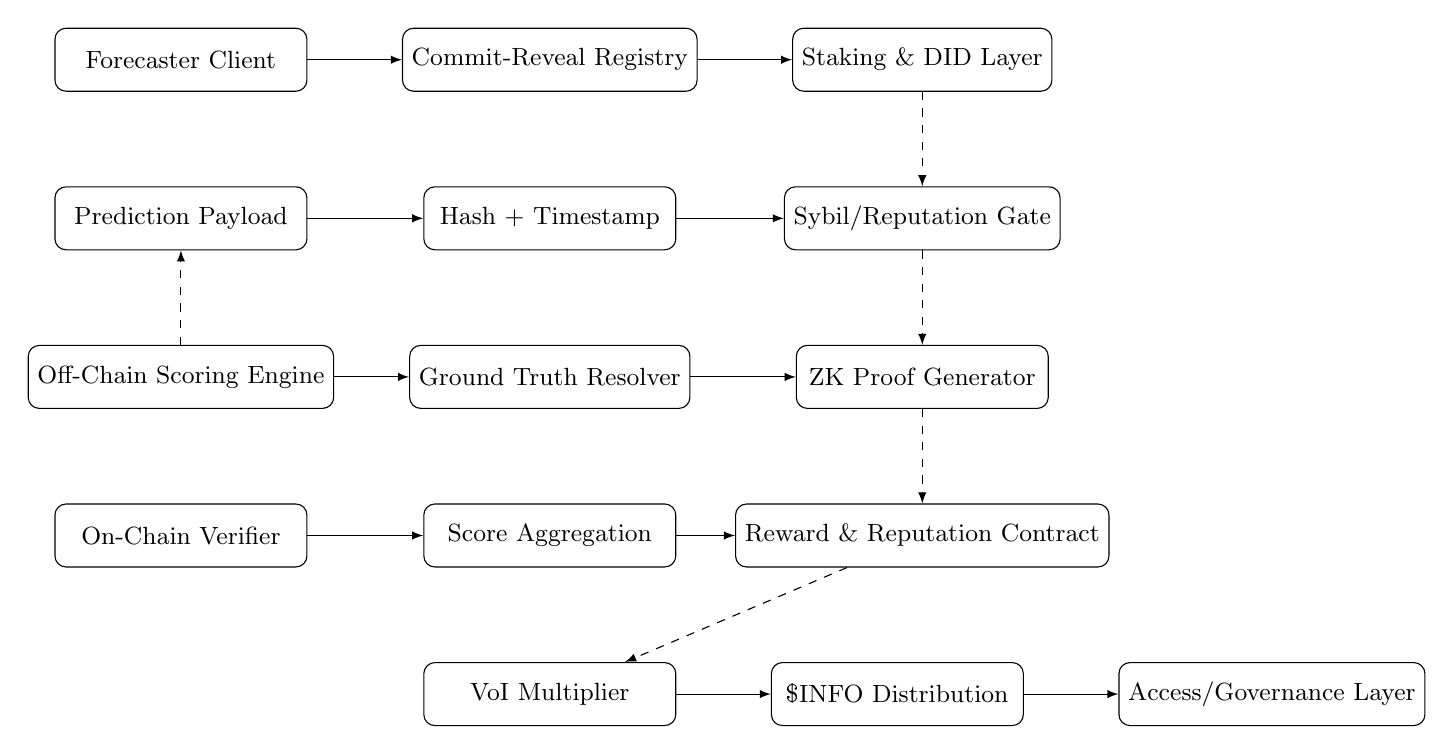
\begin{tikzpicture}[node distance=1.2cm, >=latex, box/.style={draw, rectangle, rounded corners, minimum width=3.2cm, minimum height=0.8cm, align=center, font=\small}]
    \node[box] (A) {Forecaster Client};
    \node[box, right=of A] (B) {Commit-Reveal Registry};
    \node[box, right=of B] (C) {Staking \& DID Layer};
    
    \node[box, below=of A] (D) {Prediction Payload};
    \node[box, below=of B] (E) {Hash + Timestamp};
    \node[box, below=of C] (F) {Sybil/Reputation Gate};
    
    \node[box, below=of D] (G) {Off-Chain Scoring Engine};
    \node[box, below=of E] (H) {Ground Truth Resolver};
    \node[box, below=of F] (I) {ZK Proof Generator};
    
    \node[box, below=of G] (J) {On-Chain Verifier};
    \node[box, below=of H] (K) {Score Aggregation};
    \node[box, below=of I] (L) {Reward \& Reputation Contract};
    
    \node[box, below=of K] (M) {VoI Multiplier};
    \node[box, right=of M] (N) {\$INFO Distribution};
    \node[box, right=of N] (O) {Access/Governance Layer};

    \draw[->] (A) -- (B); \draw[->] (B) -- (C);
    \draw[->] (D) -- (E); \draw[->] (E) -- (F);
    \draw[->] (G) -- (H); \draw[->] (H) -- (I);
    \draw[->] (J) -- (K); \draw[->] (K) -- (L);
    \draw[->] (M) -- (N); \draw[->] (N) -- (O);
    
    \draw[->, dashed] (C) -- (F); \draw[->, dashed] (F) -- (I);
    \draw[->, dashed] (I) -- (L); \draw[->, dashed] (G) -- (D);
    \draw[->, dashed] (L) -- (M);
\end{tikzpicture}
\captionof{figure}{InfoChain Protocol Architecture}
\end{center}

\noindent \textbf{Off-Chain/On-Chain Split:}
\begin{itemize}[leftmargin=*]
    \item \emph{Off-Chain:} Forecast aggregation, scoring computation, calibration, ZK proof generation
    \item \emph{On-Chain:} Commit-reveal registry, staking locks, proof verification, reward routing, reputation ledger
\end{itemize}

\section*{5. Core Protocol Mechanisms}
\subsection*{5.1 Commit-Reveal Flow}
\begin{enumerate}[leftmargin=*]
    \item \textbf{Commit Epoch ($t$):} Forecaster submits $H_i = \text{Keccak256}(p_i \parallel \text{salt}_i \parallel t)$
    \item \textbf{Reveal Window ($\Delta t$):} Submit $p_i, \text{salt}_i$
    \item \textbf{Late/Missing Reveal:} Stake slashed, $S_i = 0$, reputation penalized
    \item \textbf{Anti-Strategic Design:} Prevents cherry-picking, late information injection, and sybil spam
\end{enumerate}

\subsection*{5.2 Ground Truth Resolution}
Modular, economically bonded resolution:
\begin{itemize}[leftmargin=*]
    \item \textbf{Optimistic Quorum:} Multi-source median + 24--48h dispute window
    \item \textbf{Market Settlement:} Conditional token resolution (Gnosis/Polymarket)
    \item \textbf{ZK-Verified Feeds:} Cryptographically signed external data (CEX APIs, chain state)
\end{itemize}
False resolution triggers bond slashing + state rollback.

\subsection*{5.3 ZK Verification Pipeline}
\begin{enumerate}[leftmargin=*]
    \item Off-chain engine computes $S_i^{\text{norm}}$, $\mathcal{C}_i$, and reward shares
    \item Generates zk-SNARK/STARK proof using Circom/Halo2/RISC Zero
    \item On-chain verifier checks proof in $\sim$50k--150k gas (L2)
    \item Batch verification: 100--1000 forecasts per epoch
\end{enumerate}

\subsection*{5.4 Reputation \& Decay}
\begin{equation}
\text{Rep}_i^{(t)} = \alpha \cdot \text{Rep}_i^{(t-1)} + (1-\alpha) \cdot S_i^{\text{norm}}
\end{equation}
where $\alpha \in [0.8, 0.9]$ (exponential decay). Reputation gates high-stake predictions, API access tiers, and governance weight. Issued as non-transferable Soulbound Tokens (SBTs).

\section*{6. Tokenomics \& Economic Model}
\subsection*{6.1 Native Token: \texttt{\$INFO}}
\begin{center}
\begin{tabularx}{\textwidth}{@{}lX@{}}
\toprule
\textbf{Utility} & \textbf{Mechanism} \\
\midrule
Staking & Bonds forecasts; slashed for miscalibration, late reveals, collusion \\
Rewards & Distributed via scoring-weighted, VoI-adjusted pool \\
Access & Pays for high-VoI data streams, zkML forecasts, institutional APIs \\
Governance & Weighted by $\text{Rep}_i \times \text{Stake}_i$ (accuracy-adjusted voting) \\
\bottomrule
\end{tabularx}
\end{center}

\subsection*{6.2 Reward Distribution Formula}
\begin{equation}
R_i = B_t \cdot \frac{\exp(\lambda \cdot S_i^{\text{norm}})}{\sum_{j} \exp(\lambda \cdot S_j^{\text{norm}})} \cdot \left(1 - \frac{\text{Stake}_i}{\text{Stake}_{\max}}\right)^\gamma \cdot \text{VoI}_t
\end{equation}
\textbf{Default Parameters (MVP):}
\begin{itemize}[leftmargin=*]
    \item $B_t$: Protocol fees + controlled emission (adjustable per epoch)
    \item $\lambda = 4.0$ (moderate concentration; tunable via DAO)
    \item $\gamma = 0.3$ (anti-whale dampening)
    \item $\text{Stake}_{\max}$: 5\% of total staked \texttt{\$INFO}
\end{itemize}

\subsection*{6.3 Emission, Sinks \& Sustainability}
\begin{itemize}[leftmargin=*]
    \item \textbf{Sources:} L2 sequencing fees, data access subscriptions, prediction market spreads, institutional API licensing
    \item \textbf{Sinks:} Staking locks, slashing burns, reputation decay resets, protocol buybacks
    \item \textbf{Supply Model:} Utility-tied emission curve; inflation decays as protocol revenue scales. No pre-mine; fair launch via staking bootstrap.
\end{itemize}

\section*{7. Security \& Game-Theoretic Guarantees}
\begin{center}
\begin{tabularx}{\textwidth}{@{}lXX@{}}
\toprule
\textbf{Attack Vector} & \textbf{Mechanism} & \textbf{Mitigation} \\
\midrule
Sybil Farming & Low-stake trivial predictions & Capital-backed scoring, DID/SBT verification, minimum variance thresholds \\
Collusion/Cartels & Coordinated miscalibration & Diversity bonus, quadratic penalties for correlated errors, challenge periods \\
Overconfidence Gaming & Extreme $p_i$ to maximize log score & Calibration enforcement, bounded Brier fallback, isotonic regression \\
Late/Strategic Reveal & Wait for partial information & Commit-reveal windows, VRF deadlines, stake forfeiture \\
Oracle Manipulation & False ground truth resolution & Multi-source quorum, economic bonds, optimistic dispute window \\
Reward Concentration & Whales dominate payouts & Anti-whale exponent $\gamma$, dynamic $\lambda$ adjustment, reputation decay \\
\bottomrule
\end{tabularx}
\end{center}
\noindent \textbf{Game-Theoretic Guarantee:} Under strictly proper scoring + staking + commit-reveal, truthful reporting is a dominant strategy. Deviation reduces expected payoff and triggers economic penalties. Formal proof sketch provided in Appendix A.

\section*{8. Execution Roadmap}
\begin{center}
\begin{tabularx}{\textwidth}{@{}lXX@{}}
\toprule
\textbf{Development Phase} & \textbf{Deliverables} & \textbf{Tech Stack} \\
\midrule
1. Core Engine & Python/Rust scoring module, Brier/Log implementations, calibration pipeline, ABM simulation & Python, NumPy/SciPy, Mesa, Ray \\
2. Smart Contracts & Solidity commit-reveal, staking, reward distributor, reputation ledger; L2 testnet deployment & Solidity, Foundry, Arbitrum/OP testnet \\
3. ZK Verification & Circom/Halo2 circuits, proof generation pipeline, on-chain verifier audit & Circom, Halo2, SnarkJS, L2 gas optimizer \\
4. Mainnet Beta & Optimistic oracle integration, institutional API, circuit breakers, grant partnerships & Docker, CI/CD, OpenZeppelin audit, Grafana \\
\bottomrule
\end{tabularx}
\end{center}
\noindent \textbf{Deployment Prerequisites:} L2 deployment environment (Arbitrum Orbit, OP Stack, or zkSync); Foundry/Hardhat dev environment; Python simulation framework (Mesa + Monte Carlo tokenomics); ZK circuit compiler (Circom or Halo2); Test oracle resolution source (e.g., UMA, Chainlink Functions, or mock ground truth).

\section*{9. Use Cases \& Integration Paths}
\begin{enumerate}[leftmargin=*]
    \item \textbf{Next-Gen Oracle Networks:} Replace uptime/stake rewards with accuracy-calibrated payouts. Plug into Chainlink/Pyth/UMA.
    \item \textbf{AI-Agent Data Markets:} Autonomous agents stake \texttt{\$INFO} for verified, high-VoI data streams. Usage-based royalty routing.
    \item \textbf{DAO Futarchy Modules:} Policy proposals weighted by forecaster accuracy + outcome markets. Replaces plutocratic voting.
    \item \textbf{DeFi Risk Engines:} Lending/derivatives protocols consume calibrated forecast distributions for dynamic collateralization.
    \item \textbf{L2 State Optimization:} Validators rewarded for reducing fork uncertainty and improving sync efficiency.
\end{enumerate}
\noindent \textbf{Go-to-Market Wedge:} Launch as an oracle enhancement module or prediction market scoring layer on an existing L2. Partner with quant funds, AI labs, and data DAOs for initial liquidity and ground truth resolution.

\section*{10. Conclusion \& Open Research}
InfoChain Protocol reorients cryptocurrency economics from speculative value transfer to verifiable information settlement. By combining proper scoring rules, VoI-adjusted tokenomics, and ZK verification, it creates a trustless marketplace where accuracy, calibration, and uncertainty reduction are economically rewarded.

\noindent \textbf{Open Research Directions:}
\begin{itemize}[leftmargin=*]
    \item Continuous scoring rules for real-time streaming data
    \item Cross-chain VoI routing \& liquidity aggregation
    \item Regulatory-compliant data consent tokens \& audit trails
    \item zkML integration for verifiable AI forecast generation
    \item Dynamic parameter tuning via DAO governance
\end{itemize}
\noindent \textbf{Call to Action:} We invite cryptographers, mechanism designers, quant researchers, and protocol builders to contribute to the open specification, run adversarial simulations, and deploy initial modules on L2 testnets. The future of decentralized economies depends not on how much data we store, but on how well we price, verify, and act upon it.

\appendix
\section*{Appendix A: Game-Theoretic Proof Sketch}
Under strictly proper scoring $S$, expected payoff for true belief $q$ vs reported $p$:
\begin{equation}
\mathbb{E}_{x \sim q}[S(p,x)] + \mathbb{E}[\text{Stake Yield}] \leq \mathbb{E}_{x \sim q}[S(q,x)] + \mathbb{E}[\text{Stake Yield}]
\end{equation}
Slashing for miscalibration adds negative utility to deviation. Thus, truthful reporting constitutes a Nash equilibrium.

\section*{Appendix B: ZK Circuit Specification (Circom)}
\begin{itemize}[leftmargin=*]
    \item \textbf{Inputs:} \texttt{predictions[N][M]}, \texttt{outcomes[M]}, \texttt{salt[N]}, \texttt{calibration\_params}
    \item \textbf{Outputs:} \texttt{scores[N]}, \texttt{proof\_hash}
    \item \textbf{Constraints:} Keccak256 commit check, isotonic regression approximation, Brier/Log computation, reward formula bounds
    \item \textbf{Gas Target:} $<$ 150k L2 gas per batch verification
\end{itemize}

\section*{Appendix C: ABM Simulation Framework}
\begin{itemize}[leftmargin=*]
    \item \textbf{Agents:} Truthful, Overconfident, Colluding, Sybil, Late-Reveal
    \item \textbf{Metrics:} Calibration curve, Brier/log distribution, reward Gini, stake concentration, VoI scaling impact
    \item \textbf{Tools:} \texttt{Mesa} (Python), \texttt{NumPy}, \texttt{Pandas}, Monte Carlo tokenomics simulator
\end{itemize}

\section*{Appendix D: Audit \& Security Checklist}
\begin{itemize}[leftmargin=*]
    \item[$\square$] Contract formal verification (Certora or equivalent)
    \item[$\square$] ZK circuit soundness \& edge-case testing
    \item[$\square$] Economic mechanism review (game theory + ABM stress tests)
    \item[$\square$] Oracle resolution bond adequacy simulation
    \item[$\square$] Circuit breaker \& emergency pause implementation
\end{itemize}

\section*{Developer Execution Checklist}
\begin{enumerate}[leftmargin=*]
    \item[$\square$] Clone protocol repository \& set up Foundry/Halo2 environments
    \item[$\square$] Run Python ABM simulation with default parameters ($\lambda=4, \gamma=0.3, \alpha=0.85$)
    \item[$\square$] Deploy commit-reveal + staking contracts to L2 testnet
    \item[$\square$] Implement off-chain scoring engine + ZK proof generator
    \item[$\square$] Connect test oracle resolution source (mock or UMA/Chainlink)
    \item[$\square$] Run adversarial bot suite (sybil, collusion, overconfidence)
    \item[$\square$] Tune parameters based on simulation output \& gas metrics
    \item[$\square$] Request audit (contracts + ZK circuits + economic model)
    \item[$\square$] Deploy mainnet beta with circuit breakers \& transparent metrics dashboard
    \item[$\square$] Publish open datasets, calibration methods, and invite institutional partnerships
\end{enumerate}

\vspace{1em}
\noindent \textbf{License \& Contribution:} This specification is released under an open implementation license. Developers, researchers, and institutions may fork, simulate, and deploy modules under the InfoChain Architecture Framework. For code repositories, circuit audits, and simulation datasets, visit the protocol repository or join the research mailing list.

\begin{quote}
\textit{``Information is not data. Information is the reduction of uncertainty that changes decisions. InfoChain prices it, verifies it, and rewards it.''}
\end{quote}

\end{document}